\documentclass[12pt]{article}
\usepackage{amsmath} 
\usepackage{tikz}
\usetikzlibrary{positioning,shadows,arrows}
\tikzset{fact/.style={rectangle, rounded corners=1mm, draw=black,fill=green!20,drop shadow,text centered, anchor=north, text=black},
       leaf/.style={circle, draw=none, draw=black,fill=yellow!20, circular drop shadow,text centered, anchor=north, text=black}}
\begin{document}
  $$  Rownanie  Rekurencyjne  $$  
  $$   Szeregu Formalnego  $$   
 $${{a}}_{{n}} = \begin{cases}  {1}, &  \text{dla } n = 0 \\ {1}, &  \text{dla } n = 1 \\ {1}\cdot({{a}}_{{n-1}})+{1}\cdot({{a}}_{{n-2}}), &  \text{dla } n > 1 \\\end{cases} $$ $$$$ 
  
 
  $$   {{x}}_{{n}} = {1}\cdot({{x}}_{{n-1}})+{1}\cdot({{x}}_{{n-2}})$$ 
  
 
  $$ f(x) = ({{a}}_{{0}})\cdot({x}^{{0}})+({{a}}_{{1}})\cdot({x}^{{1}})+\sum_{{n} = {2}}^{{\infty}}({{a}}_{{n}})\cdot({x}^{n})$$ 
  
 
  $$    f(x) = ({{a}}_{{0}})\cdot({x}^{{0}})+({{a}}_{{1}})\cdot({x}^{{1}})+\sum_{{i} = {2}}^{{\infty}}({1}\cdot({{a}}_{{n-1}})+{1}\cdot({{a}}_{{n-2}}))\cdot({x}^{n})$$ 
 
 
 $$ f(x) = ({{a}}_{{0}})\cdot({x}^{{0}})+({{a}}_{{1}})\cdot({x}^{{1}})+\sum_{{n} = {2}}^{{\infty}}({1}\cdot({{a}}_{{n-1}}))\cdot({x}^{n})+({1}\cdot({{a}}_{{n-2}}))\cdot({x}^{n})$$ 
  
 
  $$    f(x) = ({{a}}_{{0}})\cdot({x}^{{0}})+({{a}}_{{1}})\cdot({x}^{{1}})+\sum_{{n} = {2}}^{{\infty}}({1}\cdot(({{a}}_{{n-1}})\cdot({x}^{n-1})))\cdot({x})+\sum_{{n} = {2}}^{{\infty}}({1}\cdot(({{a}}_{{n-2}})\cdot({x}^{n-2})))\cdot({x}^{2}) $$
 
 
 $$		f(x) = ({{a}}_{{0}})\cdot({x}^{{0}})+({{a}}_{{1}})\cdot({x}^{{1}})+({1}\cdot({x}))\cdot(\sum_{{j} = {1}}^{{\infty}}({{a}}_{{j}})\cdot({x}^{j}))+({1}\cdot({x}^{2}))\cdot(\sum_{{i} = {0}}^{{\infty}}({{a}}_{{i}})\cdot({x}^{i })) $$
  $$		$$ 
 $$  f(x) = ({{a}}_{{0}})\cdot({x}^{{0}})+({{a}}_{{1}})\cdot({x}^{{1}})+{1}\cdot({x})\cdot(({f(x)}-({{a}}_{{0}})))+{1}\cdot({x}^{2})\cdot({f(x)})$$ 
   $$  $$ 
   $$  {f(x)}-({1}\cdot({x})\cdot({f(x)}))-({1}\cdot({x}^{2})\cdot({f(x)}))  =  ({{a}}_{{0}})\cdot({x}^{{0}})+({{a}}_{{1}})\cdot({x}^{{1}})+{1}\cdot({x})\cdot(-({{a}}_{{0}}))$$ 
 $$  $$ 
 $$  ({f(x)})\cdot(({1}-({1}\cdot({x}))-({1}\cdot({x}^{2})))) = {{a}}_{{0}}+({x})\cdot(({{a}}_{{1}}+(-({1}))\cdot({{a}}_{{0}})\cdot({x}^{0})))$$ 
  
 
  $$ f(x) =    \frac{{{a}}_{{0}}+({x})\cdot(({{a}}_{{1}}+(-({1}))\cdot({{a}}_{{0}})\cdot({x}^{0})))}{({f(x)})\cdot(({1}-({1}\cdot({x}))-({1}\cdot({x}^{2}))))} f(x) = \frac{{{a}}_{{0}}+({x})\cdot(({{a}}_{{1}}+(-({1}))\cdot({{a}}_{{0}})\cdot({x}^{0})))}{{1}-({1}\cdot({x}))-({1}\cdot({x}^{2}))}  $$  \newpage $$    f(x) =  \frac{({1})+({x})\cdot((({1})+(-({1}))\cdot{1}\cdot{1}))}{-({1}\cdot({x}^{2}))-({1}\cdot({x}))+({1})}\delta bez skracania =  (-(({1})))^{{2}}+(-({4}))\cdot(-({1}))\cdot{1}$$\begin{center}
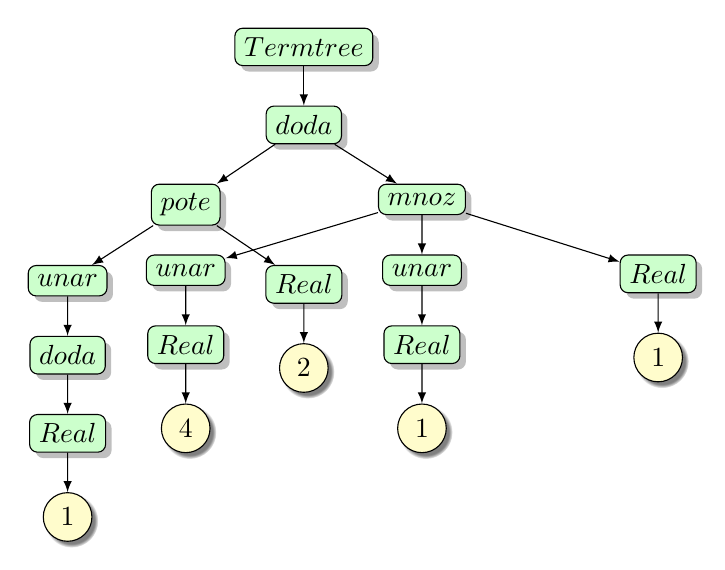
\begin{tikzpicture}[level distance=0.5cm, growth parent anchor=south]
\node [fact] {$Term tree$} [-latex]
child{ [sibling distance=3cm]
node [fact] {$doda$}
child{
node [fact] {$pote$}
child{
node [fact] {$unar$}
child{
node [fact] {$doda$}
child{
node [fact] {$Real$}
child{
node  [leaf] {$1$}
}
}
}
}
child{
node [fact] {$Real$}
child{
node  [leaf] {$2$}
}
}
}
child{
node [fact] {$mnoz$}
child{
node [fact] {$unar$}
child{
node [fact] {$Real$}
child{
node  [leaf] {$4$}
}
}
}
child{
node [fact] {$unar$}
child{
node [fact] {$Real$}
child{
node  [leaf] {$1$}
}
}
}
child{
node [fact] {$Real$}
child{
node  [leaf] {$1$}
}
}
}
};
\end{tikzpicture}
\end{center}
$ = $$({-1})^{{2}}+({4})$  $ x1 $  $ = \frac{-(-({1}))+\sqrt[{2}]{{({-1})^{{2}}+({4})}}}{{2}\cdot(-({1}))}$ $ x = \frac{({1})+\sqrt[{2}]{{({-1})^{{2}}+({4})}}}{{-2}}$  $$  x2 =  0.618034  =  \frac{({1})-(\sqrt[{2}]{{({-1})^{{2}}+({4})}})}{{-2}}$$ $$  -(\frac{({1})+\sqrt[{2}]{{({-1})^{{2}}+({4})}}}{{-2}})-(-(\frac{({1})-(\sqrt[{2}]{{({-1})^{{2}}+({4})}})}{{-2}}))$$ $$({1})+({x})\cdot((({1})+(-({1}))\cdot{1}\cdot{1}))  = \frac{{A}}{{x}-(\frac{({1})+\sqrt[{2}]{{({-1})^{{2}}+({4})}}}{{-2}})}+\frac{{B}}{{x}-(\frac{({1})-(\sqrt[{2}]{{({-1})^{{2}}+({4})}})}{{-2}})}$$  $$  ({1})+({x})\cdot((({1})+(-({1}))\cdot{1}\cdot{1}))$$ $$  =  ({x})\cdot((-({1}))\cdot{1}+(-({1}))\cdot{1})\cdot({x})  $$  $$({1})+{1}\cdot{1} = ((-({1}))\cdot{1}+(-({1}))\cdot{1})\cdot({x})({1})+({x})\cdot((({1})+(-({1}))\cdot{1}\cdot{1})) = ({x})\cdot((-({1}))\cdot{1}+(-({1}))\cdot{1})$$$$ \\ $$ \\ $$ \\ \underbrace{\left[\begin{array}{cccc}
-((-({1}))\cdot(\frac{({1})+\sqrt[{2}]{{({-1})^{{2}}+({4})}}}{{-2}})\cdot{1})&-((-({1}))\cdot(\frac{({1})-(\sqrt[{2}]{{({-1})^{{2}}+({4})}})}{{-2}})\cdot{1})& = {1}&\\
(-({1}))\cdot({A})&(-({1}))\cdot({B})& = ({1})-({1}\cdot{1})& \\
\end{array}\right]}_{M(Macierz)} \\\\ \\  $$$$ \\ $$ \\ $$ \\ \underbrace{\left[\begin{array}{cccc}
-((-({1}))\cdot(\frac{({1})+\sqrt[{2}]{{({-1})^{{2}}+({4})}}}{{-2}}))&-((-({1}))\cdot(\frac{({1})-(\sqrt[{2}]{{({-1})^{{2}}+({4})}})}{{-2}}))& = {1}&\\
(-({1}))&(-({1}))& = ({1})-({1}\cdot{1})& \\
\end{array}\right]}_{M(Macierz)} \\\\ \\   $$ $$  W1 =  -0.447214      W2  =  0.447214  $$  $$  f(x) =  \frac{{A}}{{x}-({{x}}_{{1}})}+\frac{{B}}{{x}-({{x}}_{{2}})} $$  \\ $$ $$   $$  \\ $$ $$  (\frac{{A}}{-({{x}}_{{1}})})\cdot(\sum_{{n} = {0}}^{{\infty}}\frac{{x}}{{{x}}_{{1}}}^{n})+(\frac{{B}}{-({{x}}_{{2}})})\cdot(\sum_{{n} = {0}}^{{\infty}}\frac{{x}}{{x}^{2}}^{n}) $$  \\ $$ $$   $$  \\ $$ $$   $$  \\ $$ $$   $$  \\ $$ $$  \sum_{{n} = {0}}^{{\infty}}((\frac{{0.447214}}{-({-1.61803})})\cdot(\frac{{x}}{{{x}}_{{1}}}))^{n}+\sum_{{n} = {0}}^{{\infty}}(\frac{{-0.447214}}{-({0.618034})})\cdot(\frac{{{x}}_{{1}}}{{x}^{2}}^{n}) $$  \\ $$ $$   $$  \\ $$ $$  \sum_{{n} = {0}}^{{\infty}}((\frac{{A}}{-({{x}}_{{1}})})\cdot(\frac{{x}^{n}}{{{x}}_{{1}}^{n}})+(\frac{{A}}{-({{x}}_{{1}})})\cdot(\frac{{x}^{n}}{{{x}}_{{1}}^{n}}))\cdot({x}^{n}) $$  \\ $$ $$   $$  \\ $$ $$  \sum_{{n} = {0}}^{{\infty}}({0.276393}\cdot(\frac{{1}}{{{x}}_{{1}}^{n}})+{0.723607}\cdot(\frac{{1}}{{{x}}_{{2}}^{n}}))\cdot({x}^{n}){1}$$
 
 
 $$ {1} $$ $$  Metoda Przewidywan  $$   \begin{equation}  \\ {{a}}_{{n}} = \begin{cases}  {1}, &  \text{dla } n = 0 \\ {1}, &  \text{dla } n = 1 \\ {1}\cdot({{a}}_{{n-1}})+{1}\cdot({{a}}_{{n-2}}), &  \text{dla } n > 1 \\\end{cases} \end{equation} $$ {{x}}_{{n}} = {1}\cdot({{x}}_{{{n - 1}}})+{1}\cdot({{x}}_{{{n -2}}})$$ 
  
 
  $$    {x}^{{2}} = {1}\cdot({x})+({1})$$ 
  
 
  $$    {x}^{{2}}-({1}\cdot({x}))-({1}) = 0 $$ 
  
 
      $$ \Delta   = (-({1}))^{{2}}-({4}\cdot{1}\cdot(-({1})))  $$ $$ \Delta  = ({-1})^{{2}}+({4})$$ 
  
 
      $$ \sqrt{\Delta} =  \sqrt[{2}]{{({-1})^{{2}}+({4})}} = 2.23607 $$ 
  
 
       
  
 
  $$     \ \ \\ x1 =     \frac{({1})-(\sqrt[{2}]{{({-1})^{{2}}+({4})}})}{{2}}$$ 
  
 
  $$     \     \ \\ x2 =     \frac{({1})+\sqrt[{2}]{{({-1})^{{2}}+({4})}}}{{2}}$$ 
  
 
  $$    {{f}}_{{n}}  =   ({{C}}_{{1}})\cdot(\frac{({1})-(\sqrt[{2}]{{({-1})^{{2}}+({4})}})}{{2}}^{n})+({{C}}_{{2}})\cdot(\frac{({1})+\sqrt[{2}]{{({-1})^{{2}}+({4})}}}{{2}}^{n})$$$$({{C}}_{{1}})\cdot(\frac{({1})-(\sqrt[{2}]{{({-1})^{{2}}+({4})}})}{{2}}^{0})+({{C}}_{{2}})\cdot(\frac{({1})+\sqrt[{2}]{{({-1})^{{2}}+({4})}}}{{2}}^{0})$$ 
  
 
 $$    ({{C}}_{{1}})\cdot(\frac{({1})-(\sqrt[{2}]{{({-1})^{{2}}+({4})}})}{{2}}^{1})+({{C}}_{{2}})\cdot(\frac{({1})+\sqrt[{2}]{{({-1})^{{2}}+({4})}}}{{2}}^{1})$$$$ \\ $$ \\ $$ \\ \underbrace{\left[\begin{array}{cccc}
{1}&{1}& = {1}&\\
\frac{({1})+\sqrt[{2}]{{({-1})^{{2}}+({4})}}}{{2}}&\frac{({1})-(\sqrt[{2}]{{({-1})^{{2}}+({4})}})}{{2}}& = {1}& \\
\end{array}\right]}_{M(Macierz)} \\\\ \\  w1 = 0.723607  w2 =  0.276393 $$ $$  C_1 = \frac{\frac{({1})+\sqrt[{2}]{{({-1})^{{2}}+({4})}}}{{2}}+({-1})}{\frac{({1})+\sqrt[{2}]{{({-1})^{{2}}+({4})}}}{{2}}-(\frac{({1})-(\sqrt[{2}]{{({-1})^{{2}}+({4})}})}{{2}})}$$  $$  \\  C_2 = \frac{({1})-(\frac{({1})-(\sqrt[{2}]{{({-1})^{{2}}+({4})}})}{{2}})}{\frac{({1})+\sqrt[{2}]{{({-1})^{{2}}+({4})}}}{{2}}-(\frac{({1})-(\sqrt[{2}]{{({-1})^{{2}}+({4})}})}{{2}})}$$ \ \ \\   ${{F}}_{{n}} = (\frac{\frac{({1})+\sqrt[{2}]{{({-1})^{{2}}+({4})}}}{{2}}+({-1})}{\frac{({1})+\sqrt[{2}]{{({-1})^{{2}}+({4})}}}{{2}}-(\frac{({1})-(\sqrt[{2}]{{({-1})^{{2}}+({4})}})}{{2}})})\cdot(\frac{({1})-(\sqrt[{2}]{{({-1})^{{2}}+({4})}})}{{2}}^{n})+(\frac{({1})-(\frac{({1})-(\sqrt[{2}]{{({-1})^{{2}}+({4})}})}{{2}})}{\frac{({1})+\sqrt[{2}]{{({-1})^{{2}}+({4})}}}{{2}}-(\frac{({1})-(\sqrt[{2}]{{({-1})^{{2}}+({4})}})}{{2}})})\cdot(\frac{({1})+\sqrt[{2}]{{({-1})^{{2}}+({4})}}}{{2}}^{n})$
  \end{document}
